\subsection{Критерии случайности ансамбля}

Для того, чтобы определить, является-ли расположение элементов ансамбля случайным, следует произвести генерацию элементов кластера $N_{generations}$ раз с одинаковым количеством элементов $N_{elements}$, присвоив каждому элементу кластера собственный индекс $e_{i}$, а затем исследовать закономерности расположения элементов в рамках каждого $i \in [0, N_{elements}]$, при фиксированном $j \in [0, N_{generations}]$ 

Если выборка значений случайна, то значение каждого ее элемента не должно зависеть от величины предшествующего и последующего членов. Для проверки этой независимости используется статистика являющаяся коэффициентом корреляции первого порядка
между элементами первичной выборки 
$$
r_{1, n}=\frac{n \sum_{i=1}^{n-1} x_{i} x_{i+1}-\left(\sum_{i=1}^{n} x_{i}\right)^{2}+n x_{1} x_{n}}{n \sum_{i=1}^{n} x_{i}^{2}-\left(\sum_{i=1}^{n} x_{i}\right)^{2}}
$$
являющаяся коэффициентом корреляции первого порядка
между элементами первичной выборки $ \left(x_{1}, \ldots, x_{n}\right) $ и элементами выборки, полученной из нее сдвигом на одну единицу $\left(x_{2}, x_{3}, \ldots, x_{n}, x_{1}\right)$. Величину $r_{1, n}$,
можно считать распределенной асимптотически нормально со средним $M\left(r_{1, n}\right)$ и дисперсией $D\left(r_{1, n}\right)$, где $M\left(r_{1, n}\right)=-\frac{1}{n-1}$ \newline
$D\left(r_{1, n}\right)=\frac{n(n-3)}{(n+1)(n-1)^{2}}$ Поэтому в качестве критерия случайности может рассматриваться нормализованная статистика 
$$
r_{1, n}^{*}=\frac{\left|r_{1, n}-M\left(r_{1, n}\right)\right|}{\sqrt{D\left(r_{1, n}\right)}}
$$ 
Гипотеза о случайности отклоняется при $\left|r_{1, n}^{*}\right|>\boldsymbol{u}_{1-\frac{\alpha}{2}}$.

В нашем случае можно проводить такую проверку между координатами расположения элементов.

Результаты проверки критерием автокорреляции показали, что при одинаковом начальном расположении элементов в результате перемешивания, окружности оказываются в различных местах.

Проводя эксперимент с определенным количеством окружностей и сохранив конечные положения каждой окружности в каждой генерации, можно провести тест автокорреляции. При значении квантиля стандартного нормального распределения $u_{1-\alpha/2}$, генерации случайных ансамблей с различным количеством окружностей (от $10$ до $70$) показало, что гипотеза о случайности не отклоняется. 

\newcommand{\imgsize}{6cm}
\newcommand{\imgsubdir}{autocorrelation}
\begin{figure}[h!]
    \begin{subfigure}{0.49\textwidth}
        \centering
        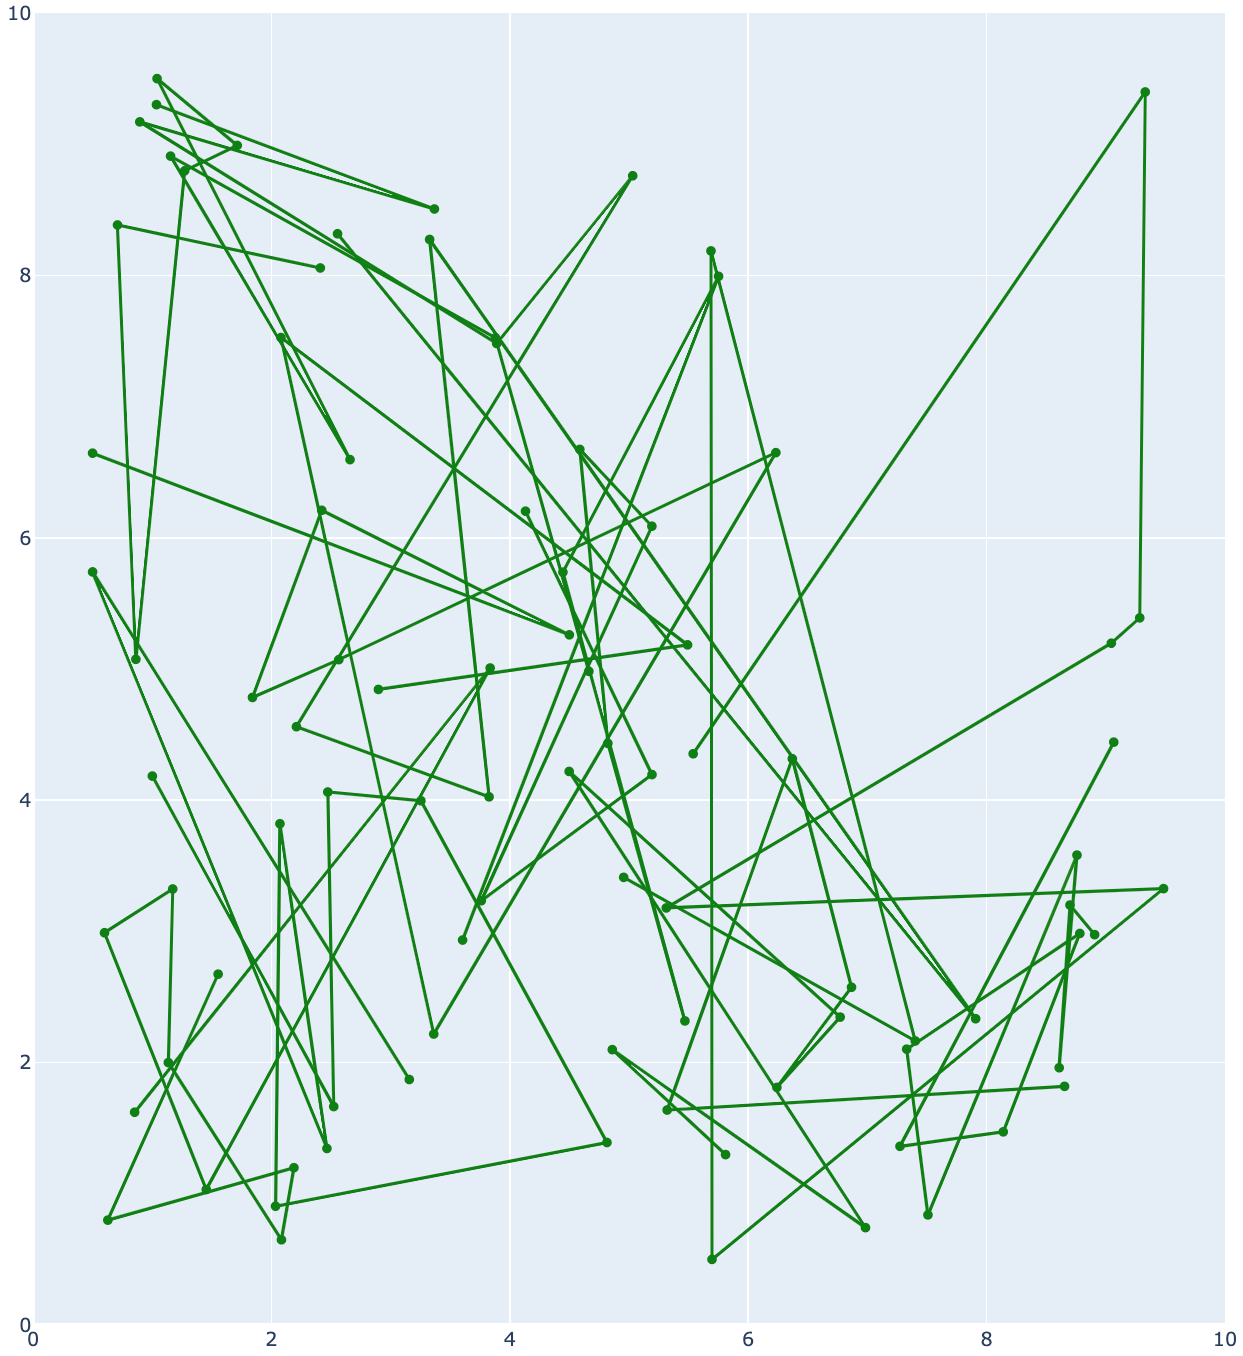
\includegraphics [width=8cm,height=\imgsize]
        {\imgdir/\imgsubdir/10c_10g_10ok.png}
        \caption{$10$ шаров, тест автокорреляции}
    \end{subfigure}
    \begin{subfigure}{0.49\textwidth}
        \centering
        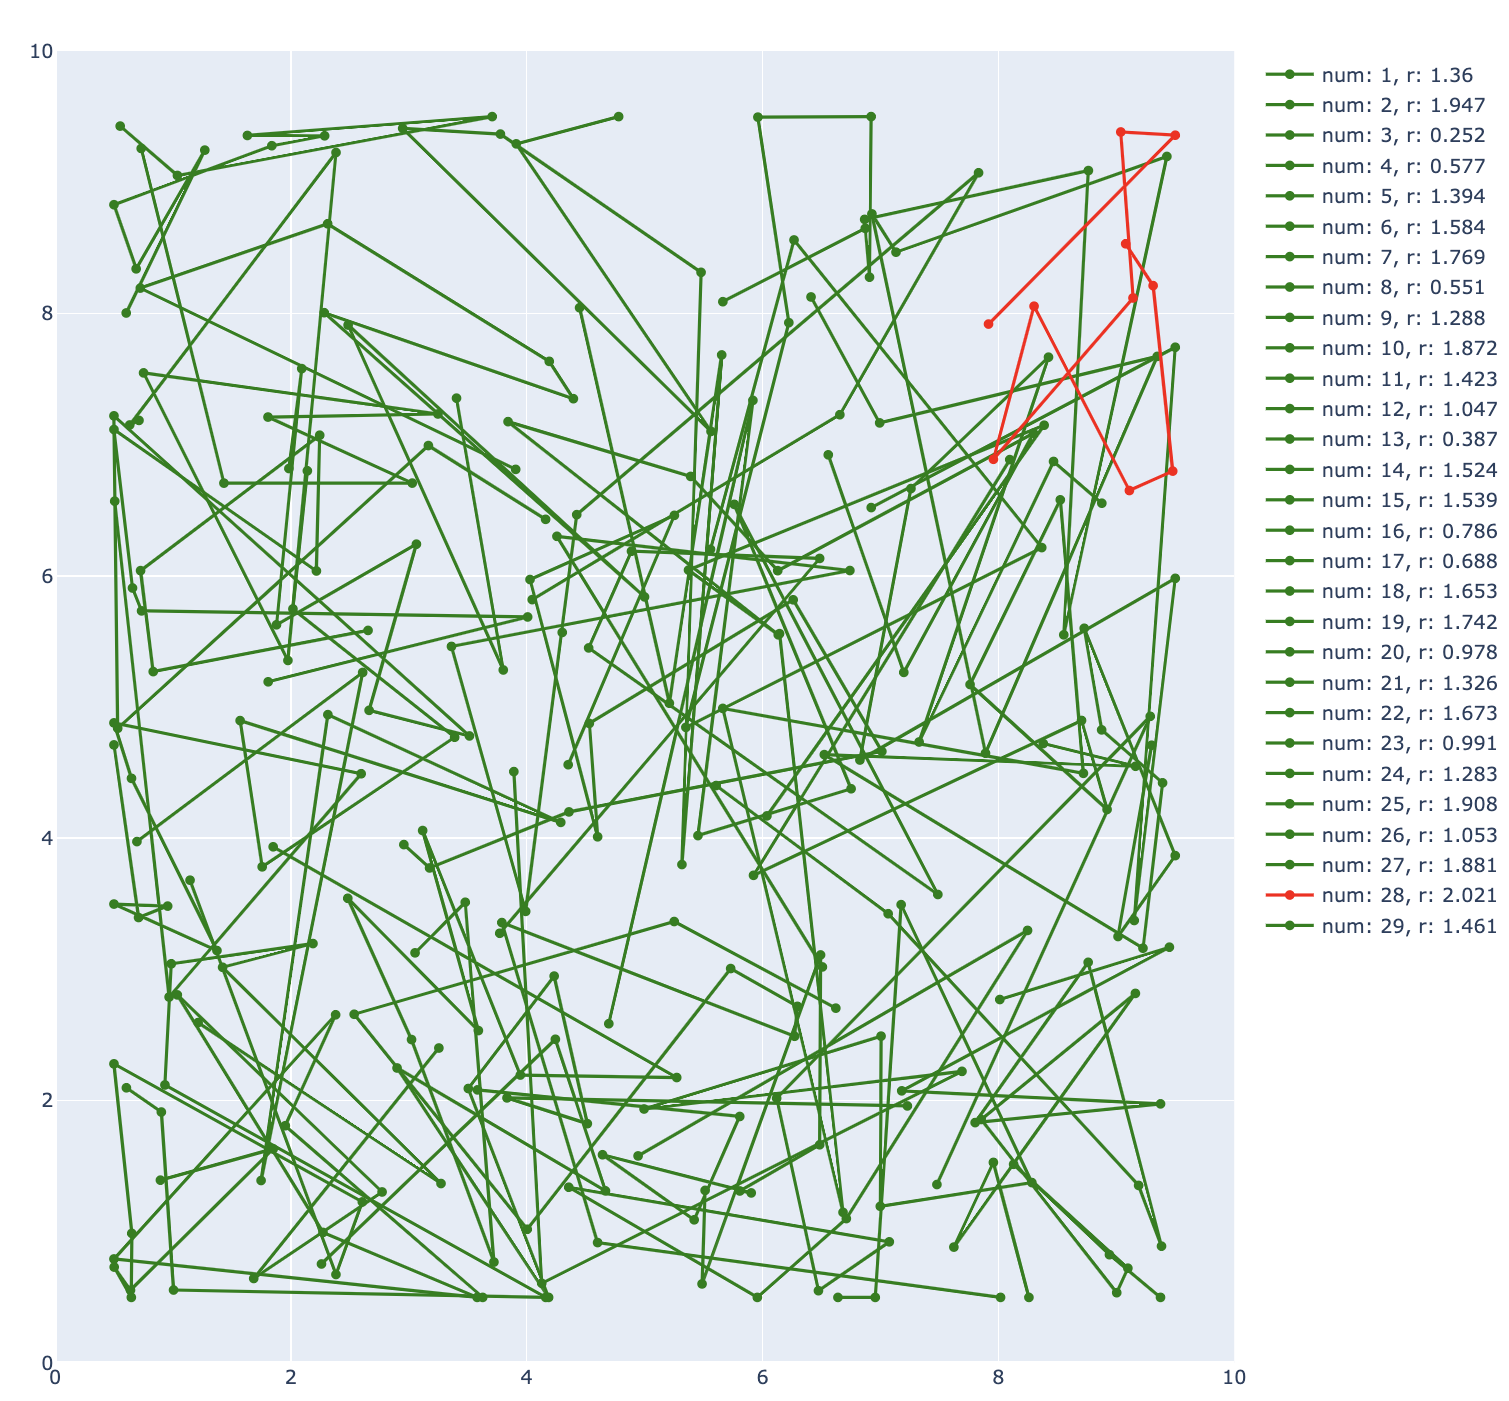
\includegraphics [width=8cm,height=\imgsize]
        {\imgdir/\imgsubdir/30c_10g_29ok.png}
        \caption{$30$ шаров, тест автокорреляции}
    \end{subfigure}
    \begin{subfigure}{0.49\textwidth}
        \centering
        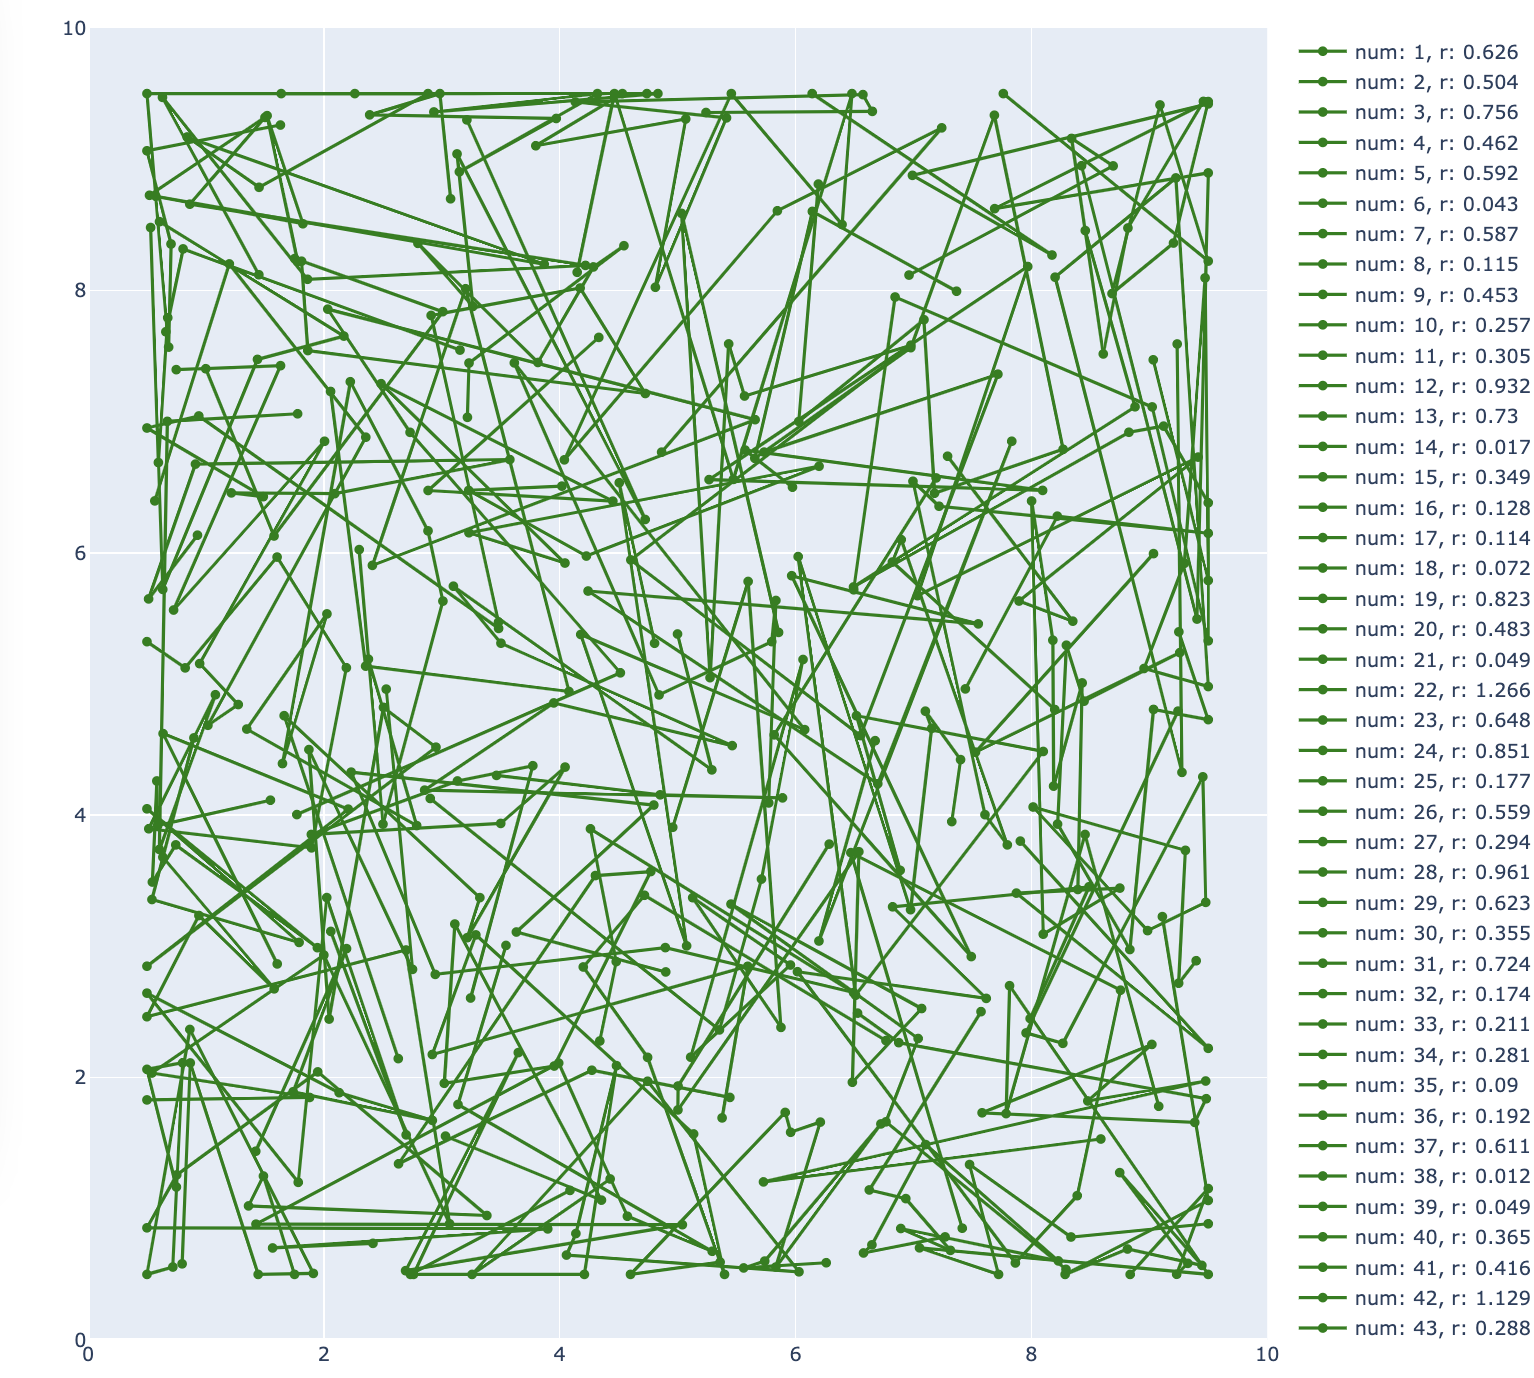
\includegraphics [width=8cm,height=\imgsize]
        {\imgdir/\imgsubdir/50c_10g_50ok.png}
        \caption{$50$ шаров, тест автокорреляции}
    \end{subfigure}
    \begin{subfigure}{0.49\textwidth}
        \centering
        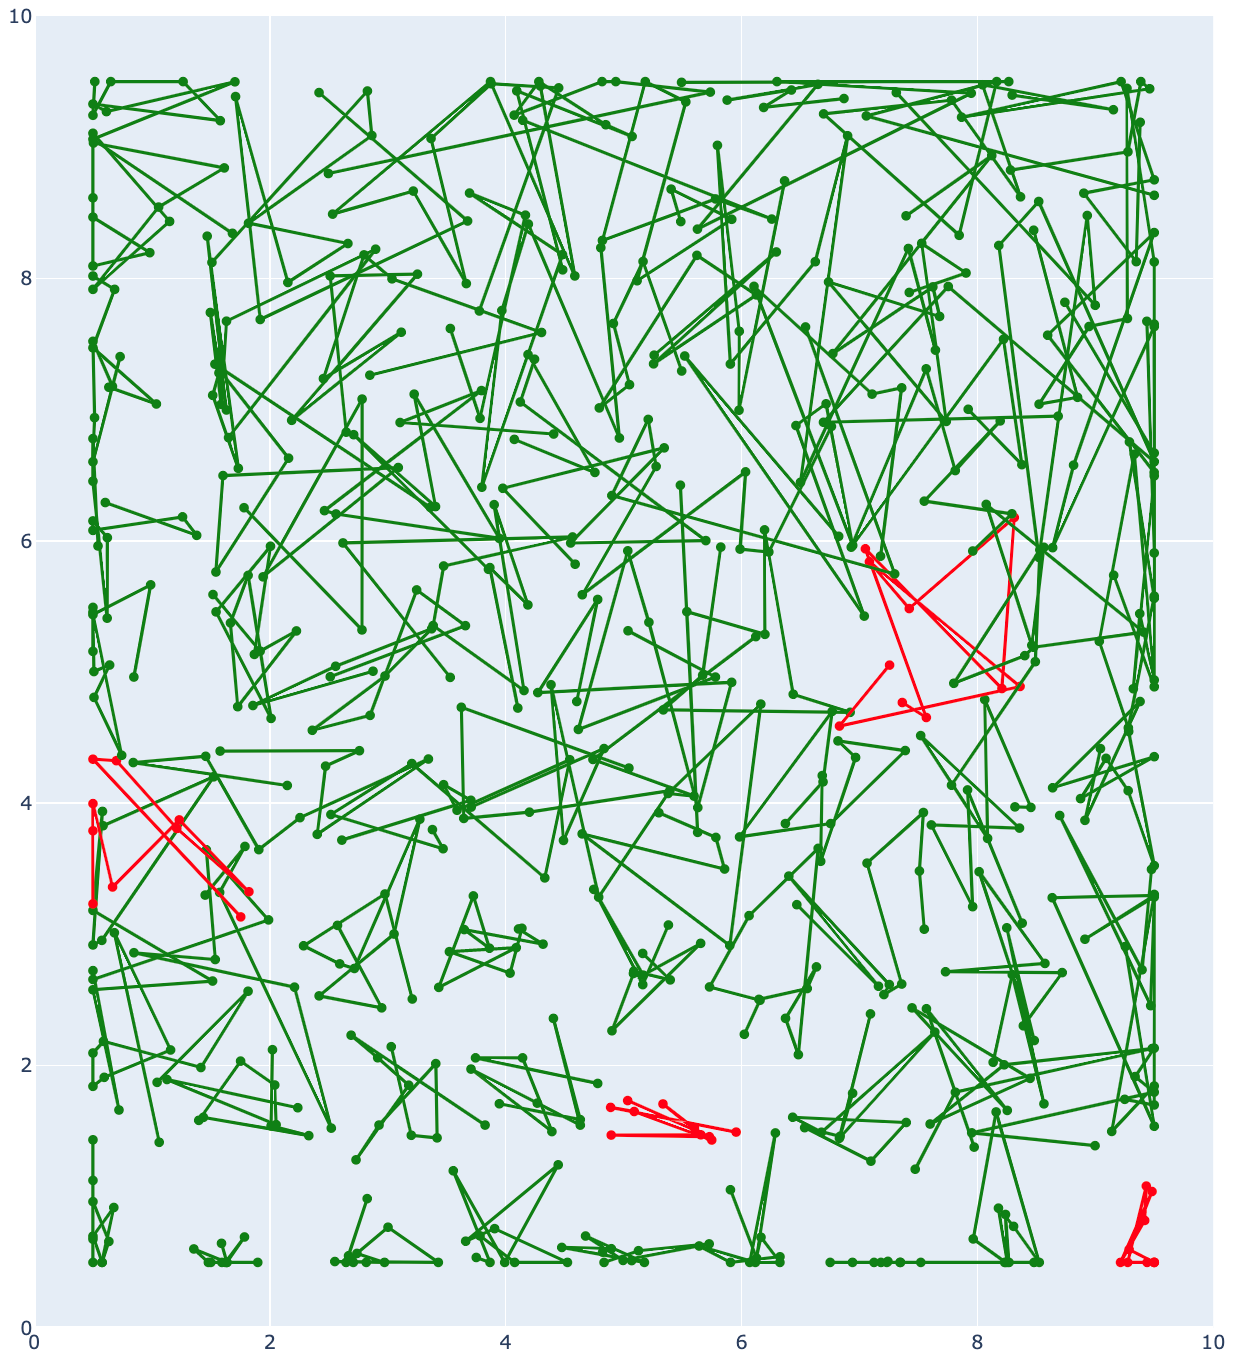
\includegraphics [width=8cm,height=\imgsize]
        {\imgdir/\imgsubdir/70c_10g_65ok.png}
        \caption{$70$ шаров, тест автокорреляции}
    \end{subfigure}
    \caption{Расположение шаров}
    \label{fig:tight_packing}
\end{figure}

